\documentclass[a4paper,11pt]{book} 

%=== PACKAGES ==============================================
\usepackage{graphicx}
\usepackage[english]{babel}
\usepackage{color}      % for colored text
\usepackage{xspace}     % for explicit spaces in abbreviations (\xspace)
\usepackage{moreverb}   % more verbatim: \begin{boxedverbatim} for source code
\usepackage{verbatim}   % for plain text
\usepackage{algorithm}  % for algorithms
\usepackage{algorithmic}% for algorithms
\usepackage{multirow}   % for multi-rows in tables
\usepackage{cite}       % will become: [2], [5]--[7]  (using cite.sty)
\usepackage{float}
\usepackage{listings}
\usepackage{array}
\usepackage{makeidx,shortvrb,latexsym}
\usepackage[latin1]{inputenc}
\usepackage{a4wide}
\usepackage{amsfonts}
\usepackage{amsmath}
\usepackage{amssymb}
%\usepackage{MnSymbol}
\usepackage{fancyhdr}
\usepackage{subfigure}
\usepackage{psfrag}
\usepackage{epsfig}
\usepackage{caption}
\usepackage{tocvsec2}
%\usepackage[draft]{pdfpages}
\usepackage{colortbl}
\usepackage[T1]{fontenc}

%% =============================================
%% LaTeX Macros 
%% =============================================
%%
%%
%% =============================================

%% -- References 
\renewcommand{\eqref}[1]{(\ref{#1})}
%\renewcommand{\eqref}[1]{Eq.~\ref{#1}}
\newcommand{\secref}[1]{Section~\ref{#1}}
\newcommand{\chapref}[1]{Chapter~\ref{#1}}
\newcommand{\figref}[1]{Fig.~\ref{#1}}
\newcommand{\tblref}[1]{Table~\ref{#1}}

%% -- soft information specific
\newcommand{\lambdaML}[1]{\ensuremath{\lambda^\mathrm{ML}_{#1}}}
\newcommand{\lambdaMLB}[1]{\ensuremath{\lambda^{\overline{\mathrm{ML}}}_{#1}}}
\newcommand{\xML}[1]{\ensuremath{x^\mathrm{ML}_{#1}}}
\newcommand{\xMLB}[1]{\ensuremath{\overline{x^\mathrm{ML}_{#1}}}}

%% -- Probabilities
\renewcommand{\Pr}[1]{\ensuremath{\mathrm{Pr}\left[#1\right]}}
\newcommand{\PDF}[1]{\ensuremath{\mathrm{p}\left(#1\right)}}
\newcommand{\Ex}{\ensuremath{\mathbb{E}}}
\newcommand{\var}[1]{\ensuremath{\mathrm{var}\left[#1\right]}}

%% -- Operators
\DeclareMathOperator*{\argmin}{arg\;min}
\DeclareMathOperator*{\argmax}{arg\;max}
\DeclareMathOperator*{\arc}{arc}
\DeclareMathOperator*{\Tr}{Tr}

%% -- Other Math
\newcommand{\dhat}{\hat{d}}
\newcommand{\xihat}{\hat{\xi}}
\newcommand{\indep}{{\;\bot\!\!\!\!\!\!\bot\;\,}}

%% -- Various commands
\newcommand{\slice}[1]{\ensuremath{\mathrm{Q}\left(#1\right)}}
\newcommand{\COrder}[1]{\ensuremath{\mathcal{O}(#1)}}
\newcommand{\vecnorm}[1]{\ensuremath{\lVert#1\rVert}}
\newcommand{\adj}[1]{\ensuremath{\mathrm{adj}\,#1}}
\newcommand{\card}[1]{\ensuremath{|#1|}}
\newcommand{\abs}[1]{\ensuremath{\left|#1\right|}}
\newcommand{\expect}[1]{\ensuremath{\mathcal{E}\{#1\}}}
\newcommand{\NP}{\ensuremath{\mathcal{NP}}}
\newcommand{\eigv}[1]{\ensuremath{\lambda(#1)}}
\newcommand{\eigvmin}[1]{\ensuremath{\lambda_{\mathrm{min}}(#1)}}
\newcommand{\eigvmax}[1]{\ensuremath{\lambda_{\mathrm{max}}(#1)}}
\newcommand{\Cdim}[2]{\ensuremath{\in\mathbb{C}^{#1\times#2}}}
\newcommand{\Rdim}[2]{\ensuremath{\in\mathbb{R}^{#1\times#2}}}
\newcommand{\with}{\ensuremath{\quad\mathrm{with}\quad}}
\newcommand{\diag}[1]{\ensuremath{\mathrm{diag}\left\lbrace#1\right\rbrace}}
\newcommand{\atan}{\ensuremath{\mathrm{atan}}}
\newcommand{\Real}{\ensuremath{\mathbb{R}}}
\newcommand{\Complex}{\ensuremath{\mathbb{C}}}
\newcommand{\cmplx}{\ensuremath{\mathsf{i}}}
\newcommand{\constant}{\ensuremath{\mathrm{const.}}}
\newcommand{\floor}[1]{\ensuremath{\lfloor#1\rfloor}}
\newcommand{\ceil}[1]{\ensuremath{\lceil#1\rceil}}
\newcommand{\round}[1]{\ensuremath{\mathrm{int}\left(#1\right)}}
\newcommand{\ltwo}{\ensuremath{\ell^{2}}}
\newcommand{\lone}{\ensuremath{\ell^{1}}}
\newcommand{\linfty}{\ensuremath{\ell^{\infty}}}

%% -- sans serif
\newcommand{\sfA}{\ensuremath{\mathsf{A}}}
\newcommand{\sfB}{\ensuremath{\mathsf{B}}}
\newcommand{\sfC}{\ensuremath{\mathsf{C}}}
\newcommand{\sfD}{\ensuremath{\mathsf{D}}}
\newcommand{\sfE}{\ensuremath{\mathsf{E}}}
\newcommand{\sfF}{\ensuremath{\mathsf{F}}}
\newcommand{\sfG}{\ensuremath{\mathsf{G}}}
\newcommand{\sfH}{\ensuremath{\mathsf{H}}}
\newcommand{\sfI}{\ensuremath{\mathsf{I}}}
\newcommand{\sfJ}{\ensuremath{\mathsf{J}}}
\newcommand{\sfK}{\ensuremath{\mathsf{K}}}
\newcommand{\sfL}{\ensuremath{\mathsf{L}}}
\newcommand{\sfM}{\ensuremath{\mathsf{M}}}
\newcommand{\sfN}{\ensuremath{\mathsf{N}}}
\newcommand{\sfO}{\ensuremath{\mathsf{O}}}
\newcommand{\sfP}{\ensuremath{\mathsf{P}}}
\newcommand{\sfQ}{\ensuremath{\mathsf{Q}}}
\newcommand{\sfR}{\ensuremath{\mathsf{R}}}
\newcommand{\sfS}{\ensuremath{\mathsf{S}}}
\newcommand{\sfT}{\ensuremath{\mathsf{T}}}
\newcommand{\sfU}{\ensuremath{\mathsf{U}}}
\newcommand{\sfV}{\ensuremath{\mathsf{V}}}
\newcommand{\sfW}{\ensuremath{\mathsf{W}}}
\newcommand{\sfX}{\ensuremath{\mathsf{X}}}
\newcommand{\sfY}{\ensuremath{\mathsf{Y}}}
\newcommand{\sfZ}{\ensuremath{\mathsf{Z}}}

%% -- Sets
\newcommand{\setA}{\ensuremath{\mathcal{A}}}
\newcommand{\setB}{\ensuremath{\mathcal{B}}}
\newcommand{\setC}{\ensuremath{\mathcal{C}}}
\newcommand{\setD}{\ensuremath{\mathcal{D}}}
\newcommand{\setE}{\ensuremath{\mathcal{E}}}
\newcommand{\setF}{\ensuremath{\mathcal{F}}}
\newcommand{\setG}{\ensuremath{\mathcal{G}}}
\newcommand{\setH}{\ensuremath{\mathcal{H}}}
\newcommand{\setI}{\ensuremath{\mathcal{I}}}
\newcommand{\setJ}{\ensuremath{\mathcal{J}}}
\newcommand{\setK}{\ensuremath{\mathcal{K}}}
\newcommand{\setL}{\ensuremath{\mathcal{L}}}
\newcommand{\setM}{\ensuremath{\mathcal{M}}}
\newcommand{\setN}{\ensuremath{\mathcal{N}}}
\newcommand{\setO}{\ensuremath{\mathcal{O}}}
\newcommand{\setP}{\ensuremath{\mathcal{P}}}
\newcommand{\setQ}{\ensuremath{\mathcal{Q}}}
\newcommand{\setR}{\ensuremath{\mathcal{R}}}
\newcommand{\setS}{\ensuremath{\mathcal{S}}}
\newcommand{\setT}{\ensuremath{\mathcal{T}}}
\newcommand{\setU}{\ensuremath{\mathcal{U}}}
\newcommand{\setV}{\ensuremath{\mathcal{V}}}
\newcommand{\setW}{\ensuremath{\mathcal{W}}}
\newcommand{\setX}{\ensuremath{\mathcal{X}}}
\newcommand{\setY}{\ensuremath{\mathcal{Y}}}
\newcommand{\setZ}{\ensuremath{\mathcal{Z}}}

%% -- Lower case letters (vectors)
\newcommand{\bma}{\ensuremath{\mathbf{a}}}
\newcommand{\bmb}{\ensuremath{\mathbf{b}}}
\newcommand{\bmc}{\ensuremath{\mathbf{c}}}
\newcommand{\bmd}{\ensuremath{\mathbf{d}}}
\newcommand{\bme}{\ensuremath{\mathbf{e}}}
\newcommand{\bmf}{\ensuremath{\mathbf{f}}}
\newcommand{\bmg}{\ensuremath{\mathbf{g}}}
\newcommand{\bmh}{\ensuremath{\mathbf{h}}}
\newcommand{\bmi}{\ensuremath{\mathbf{i}}}
\newcommand{\bmj}{\ensuremath{\mathbf{j}}}
\newcommand{\bmk}{\ensuremath{\mathbf{k}}}
\newcommand{\bml}{\ensuremath{\mathbf{l}}}
\newcommand{\bmm}{\ensuremath{\mathbf{m}}}
\newcommand{\bmn}{\ensuremath{\mathbf{n}}}
\newcommand{\bmo}{\ensuremath{\mathbf{o}}}
\newcommand{\bmp}{\ensuremath{\mathbf{p}}}
\newcommand{\bmq}{\ensuremath{\mathbf{q}}}
\newcommand{\bmr}{\ensuremath{\mathbf{r}}}
\newcommand{\bms}{\ensuremath{\mathbf{s}}}
\newcommand{\bmt}{\ensuremath{\mathbf{t}}}
\newcommand{\bmu}{\ensuremath{\mathbf{u}}}
\newcommand{\bmv}{\ensuremath{\mathbf{v}}}
\newcommand{\bmw}{\ensuremath{\mathbf{w}}}
\newcommand{\bmx}{\ensuremath{\mathbf{x}}}
\newcommand{\bmy}{\ensuremath{\mathbf{y}}}
\newcommand{\bmz}{\ensuremath{\mathbf{z}}}

%% -- Upper case letters (Matrices)
\newcommand{\bA}{\ensuremath{\mathbf{A}}}
\newcommand{\bB}{\ensuremath{\mathbf{B}}}
\newcommand{\bC}{\ensuremath{\mathbf{C}}}
\newcommand{\bD}{\ensuremath{\mathbf{D}}}
\newcommand{\bE}{\ensuremath{\mathbf{E}}}
\newcommand{\bF}{\ensuremath{\mathbf{F}}}
\newcommand{\bG}{\ensuremath{\mathbf{G}}}
\newcommand{\bH}{\ensuremath{\mathbf{H}}}
\newcommand{\bI}{\ensuremath{\mathbf{I}}}
\newcommand{\bJ}{\ensuremath{\mathbf{J}}}
\newcommand{\bK}{\ensuremath{\mathbf{K}}}
\newcommand{\bL}{\ensuremath{\mathbf{L}}}
\newcommand{\bM}{\ensuremath{\mathbf{M}}}
\newcommand{\bN}{\ensuremath{\mathbf{N}}}
\newcommand{\bO}{\ensuremath{\mathbf{O}}}
\newcommand{\bP}{\ensuremath{\mathbf{P}}}
\newcommand{\bQ}{\ensuremath{\mathbf{Q}}}
\newcommand{\bR}{\ensuremath{\mathbf{R}}}
\newcommand{\bS}{\ensuremath{\mathbf{S}}}
\newcommand{\bT}{\ensuremath{\mathbf{T}}}
\newcommand{\bU}{\ensuremath{\mathbf{U}}}
\newcommand{\bV}{\ensuremath{\mathbf{V}}}
\newcommand{\bW}{\ensuremath{\mathbf{W}}}
\newcommand{\bX}{\ensuremath{\mathbf{X}}}
\newcommand{\bY}{\ensuremath{\mathbf{Y}}}
\newcommand{\bZ}{\ensuremath{\mathbf{Z}}}
\newcommand{\bZero}{\ensuremath{\mathbf{0}}}
\newcommand{\bOne}{\ensuremath{\mathbf{1}}}
\newcommand{\bPsi}{\ensuremath{\mathbf{\Psi}}}
\newcommand{\bTheta}{\ensuremath{\mathbf{\Theta}}}
\newcommand{\bDelta}{\ensuremath{\mathbf{\Delta}}}
\newcommand{\bLambda}{\ensuremath{\mathbf{\Lambda}}}

%% -- Vectors with hat
\newcommand{\bahat}{\ensuremath{\hat{\bma}}}
\newcommand{\bbhat}{\ensuremath{\hat{\bmb}}}
\newcommand{\bchat}{\ensuremath{\hat{\bmc}}}
\newcommand{\bdhat}{\ensuremath{\hat{\bmd}}}
\newcommand{\behat}{\ensuremath{\hat{\bme}}}
\newcommand{\bfhat}{\ensuremath{\hat{\bmf}}}
\newcommand{\bghat}{\ensuremath{\hat{\bmg}}}
\newcommand{\bhhat}{\ensuremath{\hat{\bmh}}}
\newcommand{\bihat}{\ensuremath{\hat{\bmi}}}
\newcommand{\bjhat}{\ensuremath{\hat{\bmj}}}
\newcommand{\bkhat}{\ensuremath{\hat{\bmk}}}
\newcommand{\blhat}{\ensuremath{\hat{\bml}}}
\newcommand{\bmhat}{\ensuremath{\hat{\bmm}}}
\newcommand{\bnhat}{\ensuremath{\hat{\bmn}}}
\newcommand{\bohat}{\ensuremath{\hat{\bmo}}}
\newcommand{\bphat}{\ensuremath{\hat{\bmp}}}
\newcommand{\bqhat}{\ensuremath{\hat{\bmq}}}
\newcommand{\brhat}{\ensuremath{\hat{\bmr}}}
\newcommand{\bshat}{\ensuremath{\hat{\bms}}}
\newcommand{\bthat}{\ensuremath{\hat{\bmt}}}
\newcommand{\buhat}{\ensuremath{\hat{\bmu}}}
\newcommand{\bvhat}{\ensuremath{\hat{\bmv}}}
\newcommand{\bwhat}{\ensuremath{\hat{\bmw}}}
\newcommand{\bxhat}{\ensuremath{\hat{\bmx}}}
\newcommand{\byhat}{\ensuremath{\hat{\bmy}}}
\newcommand{\bzhat}{\ensuremath{\hat{\bmz}}}

%% -- Vectors with tilde
\newcommand{\batilde}{\ensuremath{\tilde{\bma}}}
\newcommand{\bbtilde}{\ensuremath{\tilde{\bmb}}}
\newcommand{\bctilde}{\ensuremath{\tilde{\bmc}}}
\newcommand{\bdtilde}{\ensuremath{\tilde{\bmd}}}
\newcommand{\betilde}{\ensuremath{\tilde{\bme}}}
\newcommand{\bftilde}{\ensuremath{\tilde{\bmf}}}
\newcommand{\bgtilde}{\ensuremath{\tilde{\bmg}}}
\newcommand{\bhtilde}{\ensuremath{\tilde{\bmh}}}
\newcommand{\bitilde}{\ensuremath{\tilde{\bmi}}}
\newcommand{\bjtilde}{\ensuremath{\tilde{\bmj}}}
\newcommand{\bktilde}{\ensuremath{\tilde{\bmk}}}
\newcommand{\bltilde}{\ensuremath{\tilde{\bml}}}
\newcommand{\bmtilde}{\ensuremath{\tilde{\bmm}}}
\newcommand{\bntilde}{\ensuremath{\tilde{\bmn}}}
\newcommand{\botilde}{\ensuremath{\tilde{\bmo}}}
\newcommand{\bptilde}{\ensuremath{\tilde{\bmp}}}
\newcommand{\bqtilde}{\ensuremath{\tilde{\bmq}}}
\newcommand{\brtilde}{\ensuremath{\tilde{\bmr}}}
\newcommand{\bstilde}{\ensuremath{\tilde{\bms}}}
\newcommand{\bttilde}{\ensuremath{\tilde{\bmt}}}
\newcommand{\butilde}{\ensuremath{\tilde{\bmu}}}
\newcommand{\bvtilde}{\ensuremath{\tilde{\bmv}}}
\newcommand{\bwtilde}{\ensuremath{\tilde{\bmw}}}
\newcommand{\bxtilde}{\ensuremath{\tilde{\bmx}}}
\newcommand{\bytilde}{\ensuremath{\tilde{\bmy}}}
\newcommand{\bztilde}{\ensuremath{\tilde{\bmz}}}

%% -- Lattices
\newcommand{\lLAMBDA}{\ensuremath{\mathbf{\Lambda}}}

%% -- MIMO specific macros
\newcommand{\MT}{\ensuremath{M_{T}}}
\newcommand{\MR}{\ensuremath{M_{R}}}
\newcommand{\SNR}{\ensuremath{\mathsf{SNR}}}
\newcommand{\SQNR}{\ensuremath{\mathrm{SQNR}}}
\newcommand{\SINR}{\ensuremath{\textsf{SINR}}}
\newcommand{\const}{\ensuremath{\setO}}
\newcommand{\mimoconst}{\ensuremath{\setO^{\MT}}}
\newcommand{\modorder}{\ensuremath{Q}}
\newcommand{\bHH}{\ensuremath{\bH^{H}}}
\newcommand{\bHbar}{\ensuremath{\bar{\bH}}}
\newcommand{\bQbar}{\ensuremath{\bar{\bQ}}}
\newcommand{\bRbar}{\ensuremath{\bar{\bR}}}
\newcommand{\bQa}{\ensuremath{\bQ_{\alpha}}}
\newcommand{\bRa}{\ensuremath{\bR_{\alpha}}}
\newcommand{\bIbar}{\ensuremath{\bar{\bI}}}
\newcommand{\bmybar}{\ensuremath{\bar{\bmy}}}
\newcommand{\bHi}{\ensuremath{\bH^{\dag}}}
\newcommand{\Pn}{\ensuremath{\sigma^{2}}}
\newcommand{\No}{\ensuremath{N_{o}}}
\newcommand{\VBLAST}{\ensuremath{\mbox{V-BLAST}}}
\newcommand{\Rate}{\ensuremath{R}}
\newcommand{\bsML}{\ensuremath{\bms^{\mathrm{ML}}}}
\newcommand{\bsZF}{\ensuremath{\bms^{\mathrm{ZF}}}}
\newcommand{\bsMMSE}{\ensuremath{\bms^{\mathrm{MMSE}}}}

%% -- VLSI things
\newcommand{\tclk}{\ensuremath{t_\mathrm{clk}}}
\newcommand{\fclk}{\ensuremath{f_\mathrm{clk}}}

%% -- Complexities
\newcommand{\CGr}{\ensuremath{C_{\mathrm{GR}}}}
\newcommand{\CVec}{\ensuremath{C_{\mathrm{Vec}}}}
\newcommand{\CRot}{\ensuremath{C_{\mathrm{Rot}}}}
\newcommand{\CMult}{\ensuremath{C_{\mathrm{Mult}}}}
\newcommand{\COMult}{\ensuremath{C_{\mathrm{OptMult}}}}
\newcommand{\CDiv}{\ensuremath{C_{\mathrm{Div}}}}
\newcommand{\CSqrt}{\ensuremath{C_{\sqrt{\cdot}}}}

%% -- NON-Math macros
\newcommand{\UMC}{$0.25\mu\mathrm{m}$ 1P/5M technology}

%% -- For NOTATION
\def\addnotation #1: #2{\parbox[t]{1.25cm}{$#1$\dotfill} \parbox[t]{3.50in}{#2} \vspace{0.0625cm} \\}
\def\addsymbol #1: #2{\parbox[t]{2cm}{$#1$} \parbox[t]{3in}{#2} \vspace{0.0625cm} \\}
\def\addacronym #1: #2{\parbox[t]{2cm}{\bf{#1}\dotfill} \parbox[t]{2.8in}{#2} \vspace{0.0625cm} \\}


\definecolor{lgray}{gray}{0.9}
\definecolor{dblue}{rgb}{0,0.08,0.7}
%\definecolor{dblue}{rgb}{0.1,0.1,0.45}
\definecolor{lred}{rgb}{1.0,0.8,0.8} 
\definecolor{lgreen}{rgb}{0.8,1.0,0.8} 

%=== Colored Hyperlinks ======================================
\usepackage[ % IF PDF
  colorlinks = true,        % links are colored
  citecolor  = dblue,        % color of cite links
  pagecolor  = dblue,        % color of page links
  linkcolor  = dblue,        % color of hyperref links
  menucolor  = dblue,        % color of Acrobat Reader menu buttons
  urlcolor   = dblue,        % color of urls \url{}
  bookmarks  = true, hyperindex=true, breaklinks=true,
  baseurl={http://www.nari.ee.ethz.ch},
  pdftitle={Distributed Multiuser Multihop Networks},             
  pdfauthor={Raphael Rolny},             
  pdfsubject={xxx},
  pdfkeywords={xxx}
]{hyperref}
    % IF LaTeX
%\usepackage[colorlinks=false]{hyperref}

%=== Theorems ================================================
\usepackage{amsthm}
\newtheorem{thm}{Theorem}[chapter]
\newtheorem{exmpl}{Example}[chapter]
\newtheorem{propos}{Proposition}[chapter]
\newtheorem{defi}{Definition}[chapter]
\newtheorem{corol}{Corollary}[chapter]
\newtheorem{lemma}{Lemma}[chapter]

%== for algorithms ============================================
\floatstyle{ruled}
\newfloat{algorithm}{tb}{loa}  % loa: auxiliary file for list of algorithms
\floatname{algorithm}{Algorithm}
\newcommand{\theHalgorithm}{\arabic{algorithm}}

%=== Index ====================================================
%\usepackage{makeidx} 
%\makeindex 

%=== Fancy header =============================================
\pagestyle{fancyplain}
% with this we ensure that the chapter and section headings are in lowercase
\fancyhf{} % delete current setting for header and footer
\fancyhead[LE,RO]{\thepage}
\fancyhead[LO]{\rightmark}
\fancyhead[RE]{\leftmark}
\addtolength{\headheight}{1.6pt} % make space for the rule
\renewcommand{\headrulewidth}{0.5pt}
\fancypagestyle{plain}{
   \fancyhead{}  % get rid of headers on plain pages
   \renewcommand{\headrulewidth}{0pt} % and the line
}


% --- Definition of short-cuts/macros ------------------------------
%%% =============================================
%% LaTeX Macros 
%% =============================================
%%
%%
%% =============================================

%% -- References 
\renewcommand{\eqref}[1]{(\ref{#1})}
%\renewcommand{\eqref}[1]{Eq.~\ref{#1}}
\newcommand{\secref}[1]{Section~\ref{#1}}
\newcommand{\chapref}[1]{Chapter~\ref{#1}}
\newcommand{\figref}[1]{Fig.~\ref{#1}}
\newcommand{\tblref}[1]{Table~\ref{#1}}

%% -- soft information specific
\newcommand{\lambdaML}[1]{\ensuremath{\lambda^\mathrm{ML}_{#1}}}
\newcommand{\lambdaMLB}[1]{\ensuremath{\lambda^{\overline{\mathrm{ML}}}_{#1}}}
\newcommand{\xML}[1]{\ensuremath{x^\mathrm{ML}_{#1}}}
\newcommand{\xMLB}[1]{\ensuremath{\overline{x^\mathrm{ML}_{#1}}}}

%% -- Probabilities
\renewcommand{\Pr}[1]{\ensuremath{\mathrm{Pr}\left[#1\right]}}
\newcommand{\PDF}[1]{\ensuremath{\mathrm{p}\left(#1\right)}}
\newcommand{\Ex}{\ensuremath{\mathbb{E}}}
\newcommand{\var}[1]{\ensuremath{\mathrm{var}\left[#1\right]}}

%% -- Operators
\DeclareMathOperator*{\argmin}{arg\;min}
\DeclareMathOperator*{\argmax}{arg\;max}
\DeclareMathOperator*{\arc}{arc}
\DeclareMathOperator*{\Tr}{Tr}

%% -- Other Math
\newcommand{\dhat}{\hat{d}}
\newcommand{\xihat}{\hat{\xi}}
\newcommand{\indep}{{\;\bot\!\!\!\!\!\!\bot\;\,}}

%% -- Various commands
\newcommand{\slice}[1]{\ensuremath{\mathrm{Q}\left(#1\right)}}
\newcommand{\COrder}[1]{\ensuremath{\mathcal{O}(#1)}}
\newcommand{\vecnorm}[1]{\ensuremath{\lVert#1\rVert}}
\newcommand{\adj}[1]{\ensuremath{\mathrm{adj}\,#1}}
\newcommand{\card}[1]{\ensuremath{|#1|}}
\newcommand{\abs}[1]{\ensuremath{\left|#1\right|}}
\newcommand{\expect}[1]{\ensuremath{\mathcal{E}\{#1\}}}
\newcommand{\NP}{\ensuremath{\mathcal{NP}}}
\newcommand{\eigv}[1]{\ensuremath{\lambda(#1)}}
\newcommand{\eigvmin}[1]{\ensuremath{\lambda_{\mathrm{min}}(#1)}}
\newcommand{\eigvmax}[1]{\ensuremath{\lambda_{\mathrm{max}}(#1)}}
\newcommand{\Cdim}[2]{\ensuremath{\in\mathbb{C}^{#1\times#2}}}
\newcommand{\Rdim}[2]{\ensuremath{\in\mathbb{R}^{#1\times#2}}}
\newcommand{\with}{\ensuremath{\quad\mathrm{with}\quad}}
\newcommand{\diag}[1]{\ensuremath{\mathrm{diag}\left\lbrace#1\right\rbrace}}
\newcommand{\atan}{\ensuremath{\mathrm{atan}}}
\newcommand{\Real}{\ensuremath{\mathbb{R}}}
\newcommand{\Complex}{\ensuremath{\mathbb{C}}}
\newcommand{\cmplx}{\ensuremath{\mathsf{i}}}
\newcommand{\constant}{\ensuremath{\mathrm{const.}}}
\newcommand{\floor}[1]{\ensuremath{\lfloor#1\rfloor}}
\newcommand{\ceil}[1]{\ensuremath{\lceil#1\rceil}}
\newcommand{\round}[1]{\ensuremath{\mathrm{int}\left(#1\right)}}
\newcommand{\ltwo}{\ensuremath{\ell^{2}}}
\newcommand{\lone}{\ensuremath{\ell^{1}}}
\newcommand{\linfty}{\ensuremath{\ell^{\infty}}}

%% -- sans serif
\newcommand{\sfA}{\ensuremath{\mathsf{A}}}
\newcommand{\sfB}{\ensuremath{\mathsf{B}}}
\newcommand{\sfC}{\ensuremath{\mathsf{C}}}
\newcommand{\sfD}{\ensuremath{\mathsf{D}}}
\newcommand{\sfE}{\ensuremath{\mathsf{E}}}
\newcommand{\sfF}{\ensuremath{\mathsf{F}}}
\newcommand{\sfG}{\ensuremath{\mathsf{G}}}
\newcommand{\sfH}{\ensuremath{\mathsf{H}}}
\newcommand{\sfI}{\ensuremath{\mathsf{I}}}
\newcommand{\sfJ}{\ensuremath{\mathsf{J}}}
\newcommand{\sfK}{\ensuremath{\mathsf{K}}}
\newcommand{\sfL}{\ensuremath{\mathsf{L}}}
\newcommand{\sfM}{\ensuremath{\mathsf{M}}}
\newcommand{\sfN}{\ensuremath{\mathsf{N}}}
\newcommand{\sfO}{\ensuremath{\mathsf{O}}}
\newcommand{\sfP}{\ensuremath{\mathsf{P}}}
\newcommand{\sfQ}{\ensuremath{\mathsf{Q}}}
\newcommand{\sfR}{\ensuremath{\mathsf{R}}}
\newcommand{\sfS}{\ensuremath{\mathsf{S}}}
\newcommand{\sfT}{\ensuremath{\mathsf{T}}}
\newcommand{\sfU}{\ensuremath{\mathsf{U}}}
\newcommand{\sfV}{\ensuremath{\mathsf{V}}}
\newcommand{\sfW}{\ensuremath{\mathsf{W}}}
\newcommand{\sfX}{\ensuremath{\mathsf{X}}}
\newcommand{\sfY}{\ensuremath{\mathsf{Y}}}
\newcommand{\sfZ}{\ensuremath{\mathsf{Z}}}

%% -- Sets
\newcommand{\setA}{\ensuremath{\mathcal{A}}}
\newcommand{\setB}{\ensuremath{\mathcal{B}}}
\newcommand{\setC}{\ensuremath{\mathcal{C}}}
\newcommand{\setD}{\ensuremath{\mathcal{D}}}
\newcommand{\setE}{\ensuremath{\mathcal{E}}}
\newcommand{\setF}{\ensuremath{\mathcal{F}}}
\newcommand{\setG}{\ensuremath{\mathcal{G}}}
\newcommand{\setH}{\ensuremath{\mathcal{H}}}
\newcommand{\setI}{\ensuremath{\mathcal{I}}}
\newcommand{\setJ}{\ensuremath{\mathcal{J}}}
\newcommand{\setK}{\ensuremath{\mathcal{K}}}
\newcommand{\setL}{\ensuremath{\mathcal{L}}}
\newcommand{\setM}{\ensuremath{\mathcal{M}}}
\newcommand{\setN}{\ensuremath{\mathcal{N}}}
\newcommand{\setO}{\ensuremath{\mathcal{O}}}
\newcommand{\setP}{\ensuremath{\mathcal{P}}}
\newcommand{\setQ}{\ensuremath{\mathcal{Q}}}
\newcommand{\setR}{\ensuremath{\mathcal{R}}}
\newcommand{\setS}{\ensuremath{\mathcal{S}}}
\newcommand{\setT}{\ensuremath{\mathcal{T}}}
\newcommand{\setU}{\ensuremath{\mathcal{U}}}
\newcommand{\setV}{\ensuremath{\mathcal{V}}}
\newcommand{\setW}{\ensuremath{\mathcal{W}}}
\newcommand{\setX}{\ensuremath{\mathcal{X}}}
\newcommand{\setY}{\ensuremath{\mathcal{Y}}}
\newcommand{\setZ}{\ensuremath{\mathcal{Z}}}

%% -- Lower case letters (vectors)
\newcommand{\bma}{\ensuremath{\mathbf{a}}}
\newcommand{\bmb}{\ensuremath{\mathbf{b}}}
\newcommand{\bmc}{\ensuremath{\mathbf{c}}}
\newcommand{\bmd}{\ensuremath{\mathbf{d}}}
\newcommand{\bme}{\ensuremath{\mathbf{e}}}
\newcommand{\bmf}{\ensuremath{\mathbf{f}}}
\newcommand{\bmg}{\ensuremath{\mathbf{g}}}
\newcommand{\bmh}{\ensuremath{\mathbf{h}}}
\newcommand{\bmi}{\ensuremath{\mathbf{i}}}
\newcommand{\bmj}{\ensuremath{\mathbf{j}}}
\newcommand{\bmk}{\ensuremath{\mathbf{k}}}
\newcommand{\bml}{\ensuremath{\mathbf{l}}}
\newcommand{\bmm}{\ensuremath{\mathbf{m}}}
\newcommand{\bmn}{\ensuremath{\mathbf{n}}}
\newcommand{\bmo}{\ensuremath{\mathbf{o}}}
\newcommand{\bmp}{\ensuremath{\mathbf{p}}}
\newcommand{\bmq}{\ensuremath{\mathbf{q}}}
\newcommand{\bmr}{\ensuremath{\mathbf{r}}}
\newcommand{\bms}{\ensuremath{\mathbf{s}}}
\newcommand{\bmt}{\ensuremath{\mathbf{t}}}
\newcommand{\bmu}{\ensuremath{\mathbf{u}}}
\newcommand{\bmv}{\ensuremath{\mathbf{v}}}
\newcommand{\bmw}{\ensuremath{\mathbf{w}}}
\newcommand{\bmx}{\ensuremath{\mathbf{x}}}
\newcommand{\bmy}{\ensuremath{\mathbf{y}}}
\newcommand{\bmz}{\ensuremath{\mathbf{z}}}

%% -- Upper case letters (Matrices)
\newcommand{\bA}{\ensuremath{\mathbf{A}}}
\newcommand{\bB}{\ensuremath{\mathbf{B}}}
\newcommand{\bC}{\ensuremath{\mathbf{C}}}
\newcommand{\bD}{\ensuremath{\mathbf{D}}}
\newcommand{\bE}{\ensuremath{\mathbf{E}}}
\newcommand{\bF}{\ensuremath{\mathbf{F}}}
\newcommand{\bG}{\ensuremath{\mathbf{G}}}
\newcommand{\bH}{\ensuremath{\mathbf{H}}}
\newcommand{\bI}{\ensuremath{\mathbf{I}}}
\newcommand{\bJ}{\ensuremath{\mathbf{J}}}
\newcommand{\bK}{\ensuremath{\mathbf{K}}}
\newcommand{\bL}{\ensuremath{\mathbf{L}}}
\newcommand{\bM}{\ensuremath{\mathbf{M}}}
\newcommand{\bN}{\ensuremath{\mathbf{N}}}
\newcommand{\bO}{\ensuremath{\mathbf{O}}}
\newcommand{\bP}{\ensuremath{\mathbf{P}}}
\newcommand{\bQ}{\ensuremath{\mathbf{Q}}}
\newcommand{\bR}{\ensuremath{\mathbf{R}}}
\newcommand{\bS}{\ensuremath{\mathbf{S}}}
\newcommand{\bT}{\ensuremath{\mathbf{T}}}
\newcommand{\bU}{\ensuremath{\mathbf{U}}}
\newcommand{\bV}{\ensuremath{\mathbf{V}}}
\newcommand{\bW}{\ensuremath{\mathbf{W}}}
\newcommand{\bX}{\ensuremath{\mathbf{X}}}
\newcommand{\bY}{\ensuremath{\mathbf{Y}}}
\newcommand{\bZ}{\ensuremath{\mathbf{Z}}}
\newcommand{\bZero}{\ensuremath{\mathbf{0}}}
\newcommand{\bOne}{\ensuremath{\mathbf{1}}}
\newcommand{\bPsi}{\ensuremath{\mathbf{\Psi}}}
\newcommand{\bTheta}{\ensuremath{\mathbf{\Theta}}}
\newcommand{\bDelta}{\ensuremath{\mathbf{\Delta}}}
\newcommand{\bLambda}{\ensuremath{\mathbf{\Lambda}}}

%% -- Vectors with hat
\newcommand{\bahat}{\ensuremath{\hat{\bma}}}
\newcommand{\bbhat}{\ensuremath{\hat{\bmb}}}
\newcommand{\bchat}{\ensuremath{\hat{\bmc}}}
\newcommand{\bdhat}{\ensuremath{\hat{\bmd}}}
\newcommand{\behat}{\ensuremath{\hat{\bme}}}
\newcommand{\bfhat}{\ensuremath{\hat{\bmf}}}
\newcommand{\bghat}{\ensuremath{\hat{\bmg}}}
\newcommand{\bhhat}{\ensuremath{\hat{\bmh}}}
\newcommand{\bihat}{\ensuremath{\hat{\bmi}}}
\newcommand{\bjhat}{\ensuremath{\hat{\bmj}}}
\newcommand{\bkhat}{\ensuremath{\hat{\bmk}}}
\newcommand{\blhat}{\ensuremath{\hat{\bml}}}
\newcommand{\bmhat}{\ensuremath{\hat{\bmm}}}
\newcommand{\bnhat}{\ensuremath{\hat{\bmn}}}
\newcommand{\bohat}{\ensuremath{\hat{\bmo}}}
\newcommand{\bphat}{\ensuremath{\hat{\bmp}}}
\newcommand{\bqhat}{\ensuremath{\hat{\bmq}}}
\newcommand{\brhat}{\ensuremath{\hat{\bmr}}}
\newcommand{\bshat}{\ensuremath{\hat{\bms}}}
\newcommand{\bthat}{\ensuremath{\hat{\bmt}}}
\newcommand{\buhat}{\ensuremath{\hat{\bmu}}}
\newcommand{\bvhat}{\ensuremath{\hat{\bmv}}}
\newcommand{\bwhat}{\ensuremath{\hat{\bmw}}}
\newcommand{\bxhat}{\ensuremath{\hat{\bmx}}}
\newcommand{\byhat}{\ensuremath{\hat{\bmy}}}
\newcommand{\bzhat}{\ensuremath{\hat{\bmz}}}

%% -- Vectors with tilde
\newcommand{\batilde}{\ensuremath{\tilde{\bma}}}
\newcommand{\bbtilde}{\ensuremath{\tilde{\bmb}}}
\newcommand{\bctilde}{\ensuremath{\tilde{\bmc}}}
\newcommand{\bdtilde}{\ensuremath{\tilde{\bmd}}}
\newcommand{\betilde}{\ensuremath{\tilde{\bme}}}
\newcommand{\bftilde}{\ensuremath{\tilde{\bmf}}}
\newcommand{\bgtilde}{\ensuremath{\tilde{\bmg}}}
\newcommand{\bhtilde}{\ensuremath{\tilde{\bmh}}}
\newcommand{\bitilde}{\ensuremath{\tilde{\bmi}}}
\newcommand{\bjtilde}{\ensuremath{\tilde{\bmj}}}
\newcommand{\bktilde}{\ensuremath{\tilde{\bmk}}}
\newcommand{\bltilde}{\ensuremath{\tilde{\bml}}}
\newcommand{\bmtilde}{\ensuremath{\tilde{\bmm}}}
\newcommand{\bntilde}{\ensuremath{\tilde{\bmn}}}
\newcommand{\botilde}{\ensuremath{\tilde{\bmo}}}
\newcommand{\bptilde}{\ensuremath{\tilde{\bmp}}}
\newcommand{\bqtilde}{\ensuremath{\tilde{\bmq}}}
\newcommand{\brtilde}{\ensuremath{\tilde{\bmr}}}
\newcommand{\bstilde}{\ensuremath{\tilde{\bms}}}
\newcommand{\bttilde}{\ensuremath{\tilde{\bmt}}}
\newcommand{\butilde}{\ensuremath{\tilde{\bmu}}}
\newcommand{\bvtilde}{\ensuremath{\tilde{\bmv}}}
\newcommand{\bwtilde}{\ensuremath{\tilde{\bmw}}}
\newcommand{\bxtilde}{\ensuremath{\tilde{\bmx}}}
\newcommand{\bytilde}{\ensuremath{\tilde{\bmy}}}
\newcommand{\bztilde}{\ensuremath{\tilde{\bmz}}}

%% -- Lattices
\newcommand{\lLAMBDA}{\ensuremath{\mathbf{\Lambda}}}

%% -- MIMO specific macros
\newcommand{\MT}{\ensuremath{M_{T}}}
\newcommand{\MR}{\ensuremath{M_{R}}}
\newcommand{\SNR}{\ensuremath{\mathsf{SNR}}}
\newcommand{\SQNR}{\ensuremath{\mathrm{SQNR}}}
\newcommand{\SINR}{\ensuremath{\textsf{SINR}}}
\newcommand{\const}{\ensuremath{\setO}}
\newcommand{\mimoconst}{\ensuremath{\setO^{\MT}}}
\newcommand{\modorder}{\ensuremath{Q}}
\newcommand{\bHH}{\ensuremath{\bH^{H}}}
\newcommand{\bHbar}{\ensuremath{\bar{\bH}}}
\newcommand{\bQbar}{\ensuremath{\bar{\bQ}}}
\newcommand{\bRbar}{\ensuremath{\bar{\bR}}}
\newcommand{\bQa}{\ensuremath{\bQ_{\alpha}}}
\newcommand{\bRa}{\ensuremath{\bR_{\alpha}}}
\newcommand{\bIbar}{\ensuremath{\bar{\bI}}}
\newcommand{\bmybar}{\ensuremath{\bar{\bmy}}}
\newcommand{\bHi}{\ensuremath{\bH^{\dag}}}
\newcommand{\Pn}{\ensuremath{\sigma^{2}}}
\newcommand{\No}{\ensuremath{N_{o}}}
\newcommand{\VBLAST}{\ensuremath{\mbox{V-BLAST}}}
\newcommand{\Rate}{\ensuremath{R}}
\newcommand{\bsML}{\ensuremath{\bms^{\mathrm{ML}}}}
\newcommand{\bsZF}{\ensuremath{\bms^{\mathrm{ZF}}}}
\newcommand{\bsMMSE}{\ensuremath{\bms^{\mathrm{MMSE}}}}

%% -- VLSI things
\newcommand{\tclk}{\ensuremath{t_\mathrm{clk}}}
\newcommand{\fclk}{\ensuremath{f_\mathrm{clk}}}

%% -- Complexities
\newcommand{\CGr}{\ensuremath{C_{\mathrm{GR}}}}
\newcommand{\CVec}{\ensuremath{C_{\mathrm{Vec}}}}
\newcommand{\CRot}{\ensuremath{C_{\mathrm{Rot}}}}
\newcommand{\CMult}{\ensuremath{C_{\mathrm{Mult}}}}
\newcommand{\COMult}{\ensuremath{C_{\mathrm{OptMult}}}}
\newcommand{\CDiv}{\ensuremath{C_{\mathrm{Div}}}}
\newcommand{\CSqrt}{\ensuremath{C_{\sqrt{\cdot}}}}

%% -- NON-Math macros
\newcommand{\UMC}{$0.25\mu\mathrm{m}$ 1P/5M technology}

%% -- For NOTATION
\def\addnotation #1: #2{\parbox[t]{1.25cm}{$#1$\dotfill} \parbox[t]{3.50in}{#2} \vspace{0.0625cm} \\}
\def\addsymbol #1: #2{\parbox[t]{2cm}{$#1$} \parbox[t]{3in}{#2} \vspace{0.0625cm} \\}
\def\addacronym #1: #2{\parbox[t]{2cm}{\bf{#1}\dotfill} \parbox[t]{2.8in}{#2} \vspace{0.0625cm} \\}
   % include standard macros
\hyphenation{func-tion-al-ity}
\hyphenation{beam-forming}

%\newenvironment{code}{\begin{quote}}{\end{quote}}
%\newcommand{\sourcecode}[1]{\texttt{#1}}
\newcommand{\norm}{\xi}

\setcounter{tocdepth}{1} % Leveltiefe in Contents

% --- ansmath ------
\DeclareMathOperator\erfc{erfc}

%%%%%%%%%%%%%%%%%%%%%%%%%%%%%%%%%%%%%%%%%%%%%%%%%%%%%%%%%%%%%%%%%%%%%
%%%% BEGIN DOCUMENT %%%%%%%%%%%%%%%%%%%%%%%%%%%%%%%%%%%%%%%%%%%%%%%%%
%%%%%%%%%%%%%%%%%%%%%%%%%%%%%%%%%%%%%%%%%%%%%%%%%%%%%%%%%%%%%%%%%%%%%

\begin{document}
\frontmatter
\title{Distributed Multiuser Multihop Networks}
\author{Marc Müller}
\date{Spring 2014}

%=== TITLE =======================================================
\begin{titlepage}
  \thispagestyle{empty}

 \begin{figure}
 \subfigure{  
\includegraphics[width=0.4\textwidth]{figures/ethlogo} } \hspace{1.5 cm}
 \subfigure{  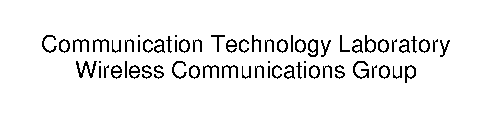
\includegraphics[width=0.5\textwidth]{figures/narilogo} }
 \end{figure}

\vspace{3 cm}
%\vspace{\stretch{20}}

\noindent
\makebox[0pt][l]{
   \begin{minipage}{\textwidth}
      \flushright{
         \huge\bfseries
         \vspace{1.5 cm}
         Optimization of MIMO Channel \\[1.2ex]
         \Large
         Subtitle of Master \\[1ex] Thesis
      }
      \noindent
      %\begin{center}
      \rule[-1ex]{\textwidth}{5pt}\\[2.5ex]      % draws black line 5pt high, \textwidth long, shifted 1ex down
      %\rule[-1ex]{\columnwidth}{5pt}\\[2.5ex]     
      %\end{center}
   \end{minipage}
}

\vspace{\stretch{7}}

 \begin{figure}[h]
 \begin{center}
 \subfigure{  
\includegraphics[width=0.5\textwidth]{figures/fertigLuschtig} } 
 \end{center}
 \end{figure}

\vspace{\stretch{8}}

\noindent
\makebox[0pt][l]{
  \begin{minipage}{\textwidth}
    \flushright{
      \bfseries 
     \large Master Thesis \\
     \normalsize Spring 2014\\
     \Large
      	\vspace{1 cm}
	%\vspace{\stretch{5}}
	Marc Müller\normalsize\\
      \vspace{0.5cm}
      Advisor:  Yahia Hassan\\ 
      Professor:  Prof. Dr. Armin Wittneben\\
      %Advisor:  J\"org Wagner\\ 
      [6ex]
	%\Large Master Thesis \normalsize \\
      %Summer 2009\\
    }
   \end{minipage}
}

\vfill

%\vspace{\stretch{1}}

\end{titlepage}

%=== Preamble ====================================================
\chapter*{Abstract}
\label{chap:abstract}
%----------------------------------------------------------
% Abstract
%----------------------------------------------------------
Here comes the abstract...

\chapter*{Preface}
\label{chap:preface}
%----------------------------------------------------------
% Preface
%----------------------------------------------------------

This Master Thesis is part of the graduate study at the Department
of Information \linebreak
Technology and Electrical Engineering (D-ITET) at the
Swiss Federal Institute of Technology (ETH) Zurich.
\\
\par The author certifies that this Master Thesis, and the research
to which it refers, are the product of the author's own work, and that
any ideas or quotations from the work of other people, published or
otherwise, are fully acknowledged in accordance with the standard
referring practices of the discipline.

\vspace{12mm}
\noindent
Muster Student
\vspace{15mm}
\begin{table}[h!]
\begin{tabular}{p{55mm}}
\hline \\
\end{tabular}
\end{table}

%----------------------------------------------------------
% Acknowledgements
%----------------------------------------------------------

\chapter*{Acknowledgements}
\label{chap:acknowledgements}

I would like to thank blablabla

\cleardoublepage

%----------------------------------------------------------
% People
%----------------------------------------------------------
\begin{center}
\begin{tabular}{l@{ }l@{\hspace{1cm}}l}
\emph{Author:} & Muster Student & student@ee.ethz.ch\\
\emph{Advisor:}& Peter Schlaumeier  & schlaumeier@nari.ee.ethz.ch\\
\emph{Professor:}& Prof. Dr. Armin Wittneben & wittneben@nari.ee.ethz.ch\\
\end{tabular}
\end{center}

\pagebreak
 % Abstract, Preface, Acknowledgements

%=== Verzeichnisse ===============================================
\tableofcontents
\listoffigures 
\listoftables
\listofalgorithms

%=== Chapters ====================================================
\mainmatter
\renewcommand{\baselinestretch}{1}\normalsize % Zeilenabstand
%\settocdepth{section} % Kapitel Sectionweise in Contents
\chapter{Information Theory}


\section{general Channel}
//by book of Tse\\
We use $x(t)$ as the transmitted signal and $y(t)$ as the received signal. Since the signal is affected by different objects in its path the received signal can be written as a function of the resulting different paths
\begin{equation}
y(t)=\sum_i{a_i(f,t)x(t-\tau_i(t))}.
\end{equation}
$a_i(f,t)$ describes the attenuation of each path which is mostly dependent on frequency and time. we can omit these dependencies if we can assume sufficient narrow bandwidth for a frequency flat channel and with relatively stationary objects a time flat channel, objects are transmitters, receivers, scatterers and so on. $\tau_i(t)$ is the delay in time of the path and is constant in a time flat channel.\\
To distinguish between these different channels we introduce some measures:
\begin{description}
	\item[Delay Spread $T_d$] describes the time difference from the first to the last arrival of the signal at the receiver.
	\item[Doppler Spread $D_s$] describes the maximum frequency difference which is introduced by Doppler shifts.
	\item[coherence Bandwidth $W_c$] is the inverse of the delay spread and a measure of the frequency flatness of the channel. It is the bandwidth at which we can assume that the channel is frequency independent.
	\item[coherence Time $T_c$] is the inverse of the Doppler spread and a measure for the time flatness of the channel e.g. it is the time over which the channel is time invariant. 
\end{description}
// image

\subsection{The equivalent baseband representation}
If we have a frequency-flat and time-flat channel we can represent our channel with a time varying channel gain $h$ which leads to 
\begin{equation}
	y(t) = h \cdot x(t)
\end{equation} for our input output relation. But it is often simpler to use a complex baseband model. if we sample the system at a sufficiently high rate we get 
\begin{equation}
	y[m] = \sum_l{h_l \cdot x[m]}
\end{equation}
where $m$ describes discrete time $x[m]$ and $y[m]$ the transmitted respectively the received signal.  

\subsection{Channel Capacity}
the channel capacity is a good figure of merit to describe the optimal performance of a communication system. It gives a maximum data rate at which we could transmit error-free when using appropriate coding.
\begin{description}
	\item[AWGN-channel:] in an AWGN channel we experience no fading and the received signal consists just the sent signal with additive white Gaussian noise $y=x+n$. The capacity depends only on the transmit $P$ versus noise Power $N_0$:
	\begin{equation}
	C=log_2\Biggr(1+\frac{P}{N_0}\Biggl) \text{     bits/s/Hz}
	\end{equation}
	\item[time- and frequency-flat fading channel:] in a one tab fading channel the capacity is a function of the tab gain $h$:
	\begin{equation}C=log_2\Biggr(1+|h|^2\frac{P}{N_0}\Biggl) \text{     bits/s/Hz}
	\end{equation}
\end{description}

\section{MIMO}
IN the thrive for higher data rates the limits of the basic single Antenna communication channels became obvious. The bandwidth limitation due to scarcity and cost and power constraints due to physics and regulations called for different approaches. MIMO uses the spatial dimension of the channel to further increase reliability and speed.

\subsection{from SISO to MIMO}
We are still using the assumptions of frequency- and time-flat channels. In the SISO case the discrete complex baseband channel tab $h$ characterized the channel sufficiently. If we now use multiple antennas an the transmitter and receiver side of the channel and make sure that they are sufficiently spaced it establishes multiple distinct channels due to small-scale fading processes. In this case our discrete complex baseband channel tab $h$ is no longer a single coefficient but a matrix $\mathbf{H}\in\mathbb{C}^{N\times M}$ with $M$ number of transmit antennas and $N$ number of receive antennas. 
\begin{equation}
	\mathbf{H} = \begin{bmatrix}
		h_{11} & h_{12} & \hdots & h_{1M} \\
		h_{21} & h_{22} & \hdots & h_{2M} \\
		\vdots & \vdots & \hdots & \vdots \\
		h_{N1} & h_{N2} & \hdots & h_{NM} \\
	\end{bmatrix}
\end{equation}

//figure \\
the input output relation of a MIMO channel is then written as 
\begin{equation}
\mathbf{y}[m] = \mathbf{Hx}[m] + \mathbf{w}[m]
\end{equation}
where $\mathbf{x}\in\mathbb{C}^M , \mathbf{y}\in\mathbb{C}^N$ and $\mathbf{w}\sim\mathcal{CN}(0,N_0\mathbf{I}_N)$


\subsection{MIMO Capacity}
the capacity of a MIMO channel without any precodeing can be written as:
\begin{equation}
	C = \log_2{\det{\Biggr[\mathbf{I}_N + \frac{\text{SNR}}{M}\mathbf{HH}^H\Biggl]}}
\end{equation}
with $\text{SNR}$ as total transmit power $P$ over noise power $N_0$.


% For a SISO channel in a Rayleigh fading channel we get a bit error rate off
% \begin{equation}
% 	P_b(|h|^2) = 1/2 \erfc{\Biggl(\sqrt{|h|^2\frac{\bar{E_b}}{N_0}}\Biggr)}.
% \end{equation}
% , if we now send the same signal over $N$ statistically independent channels we get a BER of
% \begin{equation}
% 	P_b(|h|^2) = 1/2 \erfc{\Biggl(\sqrt{\sum_{j=1}^N{|h_j|^2\frac{E_s}{N_0}}}\Biggr)}
% \end{equation}
% for the equivalent SISO channel.



\chapter{Optimization}

The question now is, is it possible to increase the Throughput of this channel with knowledge of the channel Matrix $H$. and to investigate this we use following Channel Representation and we are fully aware of its implications and imperfections.
\\// description of our channel

\section{Multiuser Case}
Since Water Filling diagonalizes the channel it does not matter what kind of decoder is used on the receiver side, the streams are already independent. But Waterfilling is only feasible in a single user case with full CSIT due to the fact that inter antenna data coordination is needed. So in a multi user scenario we need other methods to decode the channel.
We use two well-known Receiver structures:

\section{Optimizing for MMSE}
\subsection{gradient Search}

The idea of the steepest descent algorithm is to find the global maximum or minimum of a function by searching along the gradient of the function.
\begin{algorithm}
	1.	Start at one point
	2.	Calculate the Gradient
	3.	Use the gradient to get to the next point (Step)
	4.	Iterate
\end{algorithm}
We used two ways to calculate the gradient at a certain point, numerical and analytical:

\subsubsection{Numerical Gradient}
The numerical Algorithm calculates the Gradient with numerical means. Which means to increase the input in each dimension one after another by a very small amount and recalculate output. With both results, the original one and the new ones, we can approximate the local gradient very precisely.
\begin{algorithm}
	1.	Calculate Starting Point
	2.	1:K 
	a.	Increase input K
	b.	Calculate Point
	3.	Calculate Gradient
	4.	Step to next point
	5.	Iterate
\end{algorithm}
\subsubsection{Analytical Gradient}
The analytical Algorithm on the other hand uses analytical tools to calculate the gradient form the known function in advance. It uses the gradient function to calculate the exact gradient at each point.
\begin{algorithm}
	Pre: calculate analytical Gradient by hand
	1.	Calculate gradient at input Point with the precalculated gradient function
	2.	Step to the next point
	3.	Iterate
\end{algorithm}

\subsubsection{optimizing algorithm}
One Problem that occurred during the simulations was that at some point the gradient search got unstable, in our case it started to fluctuate and stopped moving towards the optimum. The reason of this bad and unwanted behavior lies in the step size of the function, and so there are two ways to fix it. The first and easy way is just to reduce the step size and increase the number of iterations accordingly, this way the problem occurs later and weaker and has less impact on the end result. The second much more complicated solution is to introduce adaptive step size.\\
Adaptive Step size means, that for each iteration we search the optimal step size which allows us to take the biggest step towards our goal. So it should not be possible to choose a step size which gives us a worse result than we had on the iteration before.
\begin{algorithm}
	Start at an arbitrary step size, calculate the next point
	If next Point is better than last, increase step size
	If next Point is worse than last, decrease step size
	Stop if increasing or decreasing does not improve the result anymore
\end{algorithm}
With this Algorithm we can prevent any fluctuation in the gradient and force it to go the fastest possible way. We do not have to calculate the gradient as often and can thus reduce the needed calculation time. Another nice side effect is, that we implicitly know that we reached the maximum or minimum when the step size is decreased to zero without finding any better points than the previous one.

\subsection{max sumRate}
To find the maximal possible and feasible throughput with a given channel matrix $\mathbf{H}$ we can optimize the sumrate with a gradient search algorithm.\\
We Optimize
\begin{equation}
	\mathbf{P} = \arg{\max_{\trace{\mathbf{P}}\leq P, p_k\geq 0\,\forall p_k\in \diag{\mathbf{P}}}{\sum_k{R}}}
\end{equation}
for a given total power $P$ so that the diagonal power allocation matrix $\mathbf{P}$ is positive-semidefinite e.g. has no negative entries.\\
The gradient search step
\begin{equation}
	\mathbf{P}^{n+1} = \mathbf{P}^n + \mu \nabla \text{sumRate}(\mathbf{P})
\end{equation}
where $(\cdot)^n$ denotes the $n$-th iteration of the search algorithm and $\mu$ an arbitrary step size.\\
We now calculate the gradient of
\begin{equation}
	\bigr\Vert{(R(\mathbf{P}))\bigl\Vert}_P = \Biggr(\sum_k{(R_k)^p}\Biggl)^{1/p}.
\end{equation}
Using the norm gives us the possibility to reuse the same calculation later for the throughput equalization (max minRate).
We know that the gradient is calculated as 
\begin{align}
	\nabla \bigr\Vert{(R(\mathbf{P}))\bigl\Vert}_P &= \nabla \Biggr[ \Biggr(\sum_k{(R_k)^p}\Biggl)^{1/p} \Biggl]\\
	&= \begin{bmatrix}
		\partial_{p_1}\\\partial_{p_2}\\\vdots\\\partial_{p_M}
	\end{bmatrix}
	\cdot \Biggr(\sum_k{(R_k)^p}\Biggl)^{1/p}
\end{align}
but first we need to convert our bounded optimization problem into an unbounded one. First to guarantee $p_k \geq 0 \, \forall k\in\diag{\mathbf{P}}$ we can introduce a diagonal matrix $\mathbf{X}$ as $x_k^2 = p_k$ with $x_k$ is the $k$-th diagonal element of $\mathbf{X}$. Secondly we need to guarantee $\trace{\mathbf{P}}\leq P$ to achieve this we tighten the condition to $\trace{\mathbf{P}}= P$.
\begin{align}
	R_k &= -\log_2\Biggr(\mathbf{\Phi}_{k,k}^{-1}\Biggl)\\
	&= -\log_2\Biggr(\biggr[ \sqrt{\mathbf{P}}\mathbf{H}^H\frac{1}{\sigma^2}\mathbf{H}\sqrt{\mathbf{P}} + \mathbf{I_M} \biggl]_{k,k}^{-1}\Biggl)\\
	&= -\log_2\Biggr(\biggr[ \sqrt{\mathbf{P} \frac{P}{\trace{\mathbf{P}}}}\mathbf{H}^H\frac{1}{\sigma^2}\mathbf{H} \sqrt{\mathbf{P} \frac{P}{\trace{\mathbf{P}}}} + \mathbf{I_M} \biggl]_{k,k}^{-1}\Biggl)\\
	&= -\log_2\Biggr(\biggr[ \mathbf{X} \sqrt{\frac{P}{\trace{\mathbf{X}^2}}} \mathbf{H}^H\frac{1}{\sigma^2}\mathbf{H} \mathbf{X} \sqrt{\frac{P}{\trace{\mathbf{X}^2}}} + \mathbf{I_M} \biggl]_{k,k}^{-1}\Biggl)\\
	&= -\log_2\Biggr(\biggr[\frac{P}{\trace{\mathbf{X}^2}} \mathbf{X}\mathbf{H}^H\frac{1}{\sigma^2}\mathbf{H} \mathbf{X} + \mathbf{I_M} \biggl]_{k,k}^{-1}\Biggl)
\end{align}
We can calculate the partial derivatives of the Rates as follows:
\begin{align}
	\partial_{x_j} \bigr\Vert{(R(\mathbf{P}))\bigl\Vert}_P
	&=\partial_{x_j}\Biggr[\Biggr(\sum_k{(R_k)^p}\Biggl)^{1/p}\Biggl]\\
	&=\frac{1}{p}\Biggr(\sum_k{(R_k)^p}\Biggl)^{1/p-1} \cdot \sum_k{\Biggr[p(R_k)^{p-1} \cdot \partial_{x_j}(R_k)\Biggl]}.
\end{align}
The partial derivative of the $k$-th users Rate $R_k$ is calculated as
\begin{align}
	\partial_{x_j}(R_k) &= \partial_{x_j}\bigr(-\log_2{\mathbf{\Phi}_{k.k}^{-1}}\bigl)\\
	&=\frac{-1}{\log{2}}\frac{1}{\mathbf{\Phi}_{k,k}^{-1}} \cdot \partial_{x_j}\bigr(\mathbf{\Phi}_{k,k}^{-1}\bigl)
\end{align}
and the derivative of the of the inverse matrix $\mathbf{\Phi}$
\begin{equation}
	\partial_{x_j}\bigr(\mathbf{\Phi}_{k,k}^{-1}\bigl) = \Biggr(-\mathbf{\Phi}^{-1} \cdot \partial_{x_j}\bigr(\mathbf{\Phi}^{-1}\bigl) \cdot \mathbf{\Phi}^{-1}\Biggl)_{k,k}.
\end{equation}
With
\begin{align}
	\partial_{x_j}\bigr(\mathbf{\Phi}^{-1}\bigl) &= \partial_{x_j} \biggr(\frac{P}{\trace{\mathbf{X}^2}} \mathbf{X}\mathbf{H}^H\frac{1}{\sigma^2}\mathbf{H} \mathbf{X} + \mathbf{I_M} \biggl)\\
	&= \partial_{x_j} \biggr(\frac{P}{\trace{\mathbf{X}^2}} \mathbf{X}\mathbf{H}^H\frac{1}{\sigma^2}\mathbf{H} \mathbf{X}\biggl)\\
	&= P \cdot \partial_{x_j} \biggr(\frac{ \mathbf{X}\mathbf{H}^H\frac{1}{\sigma^2}\mathbf{H} \mathbf{X} }{\trace{\mathbf{X}^2}}\biggl)\\
	&= P \cdot \Biggr(\frac{\partial_{x_j}\bigr(\mathbf{X}\mathbf{H}^H\frac{1}{\sigma^2}\mathbf{H}\mathbf{X}\bigl)}{\trace{\mathbf{X}^2}} - \frac{\mathbf{X}\mathbf{H}^H\frac{1}{\sigma^2}\mathbf{H}\mathbf{X} \cdot \partial_{x_j}\bigr(\trace{\mathbf{X}^2}\bigl)}{\bigr(\trace{\mathbf{X}^2}\bigl)^2}\Biggl)\\
\end{align}
and since
\begin{align}
	\partial_{x_j}\bigr(\mathbf{X}\mathbf{H}^H\frac{1}{\sigma^2}\mathbf{H}\mathbf{X}\bigl) &= \mathbf{E}_{j,j}\mathbf{H}^H\frac{1}{\sigma^2}\mathbf{HX} + \mathbf{XH}^H\frac{1}{\sigma^2}\mathbf{HE}_{j,j}\\
	\partial_{x_j}\bigr(\trace{\mathbf{X}^2}\bigl) &= 2\mathbf{XE}_{j,j}
\end{align}
it all combines together to
\begin{equation}
	\partial_{x_j}(R_k) = \frac{-1}{\log{2}}\frac{1}{\mathbf{\Phi}_{k,k}^{-1}} \cdot P \cdot \Biggr(\frac{\mathbf{E}_{j,j}\mathbf{H}^H\frac{1}{\sigma^2}\mathbf{HX} + \mathbf{XH}^H\frac{1}{\sigma^2}\mathbf{HE}_{j,j}}{\trace{\mathbf{X}^2}} - \frac{\mathbf{X}\mathbf{H}^H\frac{1}{\sigma^2}\mathbf{H}\mathbf{X} \cdot 2\mathbf{XE}_{j,j}}{\bigr(\trace{\mathbf{X}^2}\bigl)^2}\Biggl).
\end{equation}

\subsection{max minRate}
// calculations: formulas step by step\\
Implementation with the norm and not just the sum allows us to use the same function in two different ways. Firstly with a //p value of 1, we just calculate the sum Rate for the throughput maximization or sum Rate maximization. Secondly we can set the //p value to something very small like -30 to create a max-min optimizer. The Optimum would be the //min norm but this is not feasible in the numerical domain and is prone to get stuck in local minimas, here -30 is a good approximation, we tested the algorithm with -100 and achieved results which were closer to the optimum that each channel gets the same Rate but that's not save to use.
\section{optimizing VBlast}

\subsection{numeric Gradient}

\subsubsection{Numerical Gradient}
The numerical Algorithm calculates the Gradient with numerical means. Which means to increase the input in each dimension one after another by a very small amount and recalculate output. With both results, the original one and the new ones, we can approximate the local gradient very precisely.
\begin{algorithm}
	\KwIn{$\mathbf{X^{(0)}}$, $f(\mathbf{X})$, $\eta$ (interval), $\mu$ (step size)}
	\KwOut{$\mathbf{X}^{(\text{end})}$}
	\Repeat{$\nabla f(\mathbf{X}^{(n)}) = 0$}{
		\For{$k=1$ to $M$}{
			$
				\mathbf{X}_e = \mathbf{X} + \eta\mathbf{E}_{k,k}
			$\;
			$
				\partial_{X_k}(f(\mathbf{X}^{(n)}) = \frac{f(\mathbf{X}^{(n)}-f(\mathbf{X}_e)}{\eta}
			$\;
		}
		$
			\mathbf{X}^{(n+1)}=\mathbf{X}^{(n)}-\mu
			\begin{bmatrix}
				\partial_{X_1}(f(\mathbf{X}^{(n)}))\\
				\partial_{X_2}(f(\mathbf{X}^{(n)}))\\
				\vdots\\
				\partial_{X_M}(f(\mathbf{X}^{(n)}))
			\end{bmatrix}
		$\;
	}		
\end{algorithm}
\subsubsection{max sumRate}
\subsubsection{max minRate}


\section{minimize the total power for per user SINR targets}
The idea is to fix SINR targets for each user $\text{SINR}_{tgt_k}$ and then find the minimum required sum power $P_{tot} = \sum_k{P_k}$ to reach these targets. We no longer care about an upper bound for $P_{tot}$ and as always will not introduce a per user power constraint.
\begin{equation}
	\begin{aligned}
		& \underset{\mathbf{P}}{\text{minimize}}
		& & \sum_k{P_k} \\
		& \text{subject to}
		& & \text{SINR}_k = \text{SINR}_{tgt_k},\,\forall k\in K, \\
		&&& P_k\geq 0,\,\forall P_k\in \diag{\mathbf{P}}.
	\end{aligned}
\end{equation}
The channel will again be
\begin{equation}
	\mathbf{y}^{(M\times 1)} = \mathbf{H}^{(M\times K)}\cdot \mathbf{x}^{(K\times 1)}.
\end{equation}
and we will only use the LMMSE receiver.

\subsection{Fodor}
Fodor extends the work of //paper which offer a closed form solution for the above optimization problem but only works for feasible SINR targets. He proposes following algorithm:
\begin{algorithm}
	\KwIn{$t=0$, $\epsilon^{(0)}=1$, SINR targets $\mathbf{\Gamma} = \diag{\gamma_k^{tgt}}$ and transmission powers $\mathbf{P}^{(0)}$}
	\Repeat{$\mathbf{P}^{(n)}=\mathbf{P}^{(n-1)}$}{
		calculate the effective interference for MMSE processing:
		\begin{algomathdisplay}
			\begin{aligned}
				\zeta_{k,s} = \Biggl\{\Biggl(d^{-\rho}_{k,k}\chi_{k,k}\mathbf{H}^H_{k,k}&\biggl(\sum_{j\neq k}{P_jd^{-\rho}_{k,j}\chi_{k,j}\mathbf{H}_{k,j}\mathbf{T}_j\mathbf{T}_j^H\mathbf{H}^H_{k,j}}\\
				&+N\sigma^2_n\mathbf{I}\biggr)^{-1}\mathbf{H}_{k,k}+\frac{1}{P_k}\mathbf{I}\Biggr)^{-1}\Biggr\}^{(s,s)}
			\end{aligned}	
		\end{algomathdisplay}
		calculate the optimal loading matrix
		\begin{algomathdisplay}
			(\mathbf{T}_k)^{(s,s)} = \sqrt{\frac{\zeta_{k,s}N}{\sum_{j=1}^{N}\zeta_{k,j}}}\;\forall s\in[1,N]
		\end{algomathdisplay}
		calculate used Power
		\begin{equation*}
			P_k = \frac{\zeta_{k,s}}{\vert(\mathbf{T}_k)^{(s,s)}\vert^2}(\gamma_{tgt}+1)\;\forall k;
		\end{equation*}
	}
\end{algorithm}
In our single antenna per user case the precoding matrix $\mathbf{T}_k \in \mathbb{C}^{(N\times N)}$ with $\sum_{s=1}^N{|\mathbf{T}_k^{(s,s)}|^2}=N$ will always be one. $\mahtbf{H}_{k,k}$ denotes the channel matrix from user $k$ to receiver $k$ in our case we only have one base station and thus $\mathbf{H}_{k,j} \in \mathbb{C}^{(M\times 1)}$ with $j=1$. In addition we set both the distance $d^{-\rho}_{k,k}=1$ and the fading coefficient $\chi_{k,k}=1$ since we ignore path losses.

\subsection{analytical gradient}
Again we like to compare the results with a analytical gradient search algorithm. So let us first calculate the gradient for the power minimization.
The idea here was to minimize the difference between the target Rates and the calculated rate for the channel, only by changing the diagonal Values of $\mathbf{P}$.
So our minimization problem is
\begin{equation}
	\begin{aligned}
		& \underset{\mathbf{P}}{\text{minimize}}
		& & \sum_k{\bigr(R_k-R_{tgt}\bigl)} \\
		& \text{subject to}
		& & P_k\geq 0,\,\forall P_k\in \diag{\mathbf{P}}.
	\end{aligned}
\end{equation}
Again we use $\mathbf{X}^2 = \mathbf{P}$ to make sure to only get positive power Values but since we do not care about some power power budget $P_{tot}$ we can removed the condition $\trace{\mathbf{P}}\leq P_{tot}$. $\mathbf{\Phi}$ then becomes
\begin{equation}
	\mathbf{\Phi} = \mathbf{X}\mathbf{H}^H\frac{1}{\sigma^2}\mathbf{H} \mathbf{X} + \mathbf{I_N}
\end{equation}
and the for the Rate of user $k$
\begin{equation}
	R_k = -\log_2\Biggr(\mathbf{\Phi}_{k,k}^{-1}\Biggl) = -\log_2\Biggr(\biggr[\mathbf{X}\mathbf{H}^H\frac{1}{\sigma^2}\mathbf{H} \mathbf{X} + \mathbf{I_M} \biggl]_{k,k}^{-1}\Biggl)
\end{equation}
With $p=2$ we calculate the distance such that the sign does not mess up the gradient and the norm to be able to reuse the code from the throughput maximization algorithm, we get:
\begin{equation}
	\nabla \bigr\Vert{(R(\mathbf{P}))\bigl\Vert}_2 = \nabla \Biggr[ \Biggr(\sum_k{(R_k-R_{tgt})^2}\Biggl)^{1/2} \Biggl]
\end{equation}
and for the partial derivative
\begin{align}
	\partial_{x_j} \bigr\Vert{(R(\mathbf{P}))\bigl\Vert}_2
	&=\partial_{x_j}\Biggr[\Biggr(\sum_k{(R_k-R_{tgt})^2}\Biggl)^{1/2}\Biggl]\\
	&=\frac{1}{2}\Biggr(\sum_k{(R_k-R_{tgt})^2}\Biggl)^{-1/2} \cdot \sum_k{\Biggr[2(R_k-R_{tgt}) \cdot \partial_{x_j}(R_k-R_{tgt})\Biggl]}.
\end{align}
where
\begin{align}
	\partial_{x_j}(R_k-R_{tgt}) &= \partial_{x_j}(R_k)\\
	&= \partial_{x_j}\bigr(-\log_2{\mathbf{\Phi}_{k.k}^{-1}}\bigl)\\
	&=\frac{-1}{\log{2}}\frac{1}{\mathbf{\Phi}_{k,k}^{-1}} \cdot \partial_{x_j}\bigr(\mathbf{\Phi}_{k,k}^{-1}\bigl)
\end{align}
\begin{equation}
	\partial_{x_j}\bigr(\mathbf{\Phi}_{k,k}^{-1}\bigl) = \Biggr(-\mathbf{\Phi}^{-1} \cdot \partial_{x_j}\bigr(\mathbf{\Phi}^{-1}\bigl) \cdot \mathbf{\Phi}^{-1}\Biggl)_{k,k}.
\end{equation}
and the derivative of $\mathbf{\Phi}$ as
\begin{align}
	\partial_{x_j}\bigr(\mathbf{\Phi}^{-1}\bigl) &= \partial_{x_j} \biggr(\mathbf{X}\mathbf{H}^H\frac{1}{\sigma^2}\mathbf{H} \mathbf{X} + \mathbf{I_M} \biggl)\\
	&= \partial_{x_j} \biggr(\mathbf{X}\mathbf{H}^H\frac{1}{\sigma^2}\mathbf{H} \mathbf{X}\biggl)\\
	&= \mathbf{E}_{j,j}\mathbf{H}^H\frac{1}{\sigma^2}\mathbf{HX} + \mathbf{XH}^H\frac{1}{\sigma^2}\mathbf{HE}_{j,j}
\end{align}
and finally the partial derivative of $R_k$ by the $j$-th element of $\mathbf{P}$
\begin{equation}
	\begin{aligned}
		\partial_{X_j}(R_k) = &\Biggr(\sum_k{(R_k-R_{tgt})^2}\Biggl)^{-1/2}\cdot\sum_k{\Biggr[\frac{R_k-R_{tgt}}{\log{2}\cdot\mathbf{\Phi}_{k,k}^{-1}}\cdot\\&\cdot\Biggr(\mathbf{\Phi}^{-1} \cdot\Biggr( \mathbf{E}_{j,j}\mathbf{H}^H\frac{1}{\sigma^2}\mathbf{HX} + \mathbf{XH}^H\frac{1}{\sigma^2}\mathbf{HE}_{j,j}\Biggl) \cdot \mathbf{\Phi}^{-1}\Biggl)_{k,k}\Biggl]}.
	\end{aligned}
\end{equation}

\chapter{results}

%=== Appendix ===================================================
%\settocdepth{chapter} % Appendix nur Kapitelweise in Contents
\appendix
%\input{chapters/a-cdcontents}

%=== Bibliography ===============================================
%\nocite{*}
\cleardoublepage
\addcontentsline {toc}{chapter}{Bibliography} 
\bibliographystyle{IEEEtran}
\bibliography{IEEEabrv,report}
\cleardoublepage

%=== Index ======================================================
%\addcontentsline{toc}{chapter}{Index}
%\printindex 
%\cleardoublepage
\end{document}

%%%%%%%%%%%%%%%%%%%%%%%%%%%%%%%%%%%%%%%%%%%%%%%%%%%%%%%%%%%%%%%%%%%%
%%%  the  E N D  %%%%%%%%%%%%%%%%%%%%%%%%%%%%%%%%%%%%%%%%%%%%%%%%%%%
%%%%%%%%%%%%%%%%%%%%%%%%%%%%%%%%%%%%%%%%%%%%%%%%%%%%%%%%%%%%%%%%%%%%
